\documentclass[11pt,a4paper]{article}
\usepackage[utf8]{inputenc}
\usepackage{amsmath,amssymb,amsfonts}
\usepackage{geometry}
\geometry{a4paper, margin=1in}
\usepackage{booktabs}
\usepackage{graphicx}
\usepackage{microtype}
\usepackage{charter}
\usepackage[colorlinks=true, linkcolor=blue, citecolor=blue, urlcolor=blue]{hyperref}

\title{\textbf{VWAP Alpha Strategy -- Execution \& Capacity Study}}
\author{\textbf{Quantitative Research Division} \\ Confidential -- Proprietary Research}
\date{July 2026}

\begin{document}

\maketitle

\begin{abstract}
This paper presents the empirical research and operational design of the VWAP Alpha Strategy. We evaluate the capacity scaling limits and execution tradeoffs of an overnight overreaction anomaly signal in the Russell 3000 universe since 1998. We show that 3-hour VWAP execution balances market impact against alpha decay, establishing a terminal capacity ceiling of \$2.5M--\$3.0M AUM under a 1.0x leveraged margin structure.
\end{abstract}

\section{Executive Summary}
The VWAP Alpha Strategy exploits overnight overreaction anomalies to deliver institutional-grade returns. Across a 28-year historical horizon (1998--2026), the strategy achieves a Net Sharpe range of $1.30$ to $2.75$ and an unleveraged Net CAGR range of $35.13\%$ to $450.84\%$. We show that the strategy is scalable to a terminal capacity ceiling of \$2.5M--\$3.0M AUM, dictated by the market impact of liquid micro-cap stocks.

\section{Strategy Overview}
The strategy exploits overnight overreaction anomalies driven by liquidity provision imbalances, retail herd behavior, and leverage-induced liquidations during the daytime session. The signal is a cross-sectional long-only equity rank derived from the deviation between an intraday mid-price proxy and the close price, normalized by volume activity and intraday dispersion.

\section{Portfolio Construction}
The portfolio holds the Top 4 stocks selected daily, rebalanced across 3 independent rolling tranches to reduce daily turnover by $67\%$. Position weights are allocated using Inverse Volatility weighting. To mitigate execution fill risks, a soft liquidity floor of \$50K ADDV is applied below \$100K AUM, shifting to \$1M ADDV above \$100K AUM.

\begin{table}[htbp]
\centering
\caption{Soft Liquidity Floor Comparison (2020--2026)}
\begin{tabular}{llccc}
\toprule
AUM Scale & Liquidity Filter & Net Sharpe & Net CAGR & Max Drawdown \\
\midrule
\$1K & None (Baseline) & 2.382 & 263.42\% & -47.78\% \\
\$1K & \textbf{\$50K DADV Floor} & \textbf{2.218} & \textbf{228.37\%} & \textbf{-50.84\%} \\
\$1K & \$100K DADV Floor & 2.115 & 203.39\% & -50.65\% \\
\midrule
\$10K & None (Baseline) & 2.345 & 255.22\% & -48.07\% \\
\$10K & \textbf{\$50K DADV Floor} & \textbf{2.193} & \textbf{223.39\%} & \textbf{-51.04\%} \\
\$10K & \$100K DADV Floor & 2.092 & 199.16\% & -50.82\% \\
\midrule
\$100K & None (Baseline) & 2.228 & 230.48\% & -48.97\% \\
\$100K & \textbf{\$50K DADV Floor} & \textbf{2.115} & \textbf{208.14\%} & \textbf{-51.69\%} \\
\$100K & \$100K DADV Floor & 2.018 & 186.16\% & -51.35\% \\
\bottomrule
\end{tabular}
\end{table}

\section{Execution Model}
Exits are routed via a 3-hour VWAP execution horizon. Slicing reduces price impact but exposes the trade to morning-session alpha decay. The net return is modeled as a strictly concave function of execution duration $H$:
\begin{equation}
\text{Net Return}(H) = \text{Gross Alpha} - a \cdot H - \frac{b}{H}
\end{equation}
Taking the second derivative:
\begin{equation}
\frac{d^2(\text{Net Return})}{dH^2} = -\frac{2b}{H^3} < 0
\end{equation}
proving a unique global maximum at $H^* = 3.0$ hours.

\section{Capacity Analysis}
The terminal capacity ceiling is \$2.5M--\$3.0M AUM. Past this point, the non-linear market impact of trading \$1M ADV stocks dominates the alpha, causing drawdowns to spike to near $-80\%$.

\begin{table}[htbp]
\centering
\caption{Full Horizon Performance Metrics (1998--2026)}
\begin{tabular}{lcccc}
\toprule
AUM Scale & Net Sharpe & Net CAGR & Max Drawdown & Status \\
\midrule
\$10K & 2.571 & 386.36\% & -48.07\% & Safe \\
\$100K & 1.652 & 96.12\% & -55.19\% & Safe \\
\$1.0M & 1.463 & 79.34\% & -57.45\% & Safe \\
\$2.5M & 1.303 & 66.21\% & -64.44\% & Terminal \\
\$10.0M & 0.866 & 35.13\% & -78.20\% & Over-capacity \\
\bottomrule
\end{tabular}
\end{table}

\section{Strategy Equity Curves (PnL)}
We plot the cumulative performance of the strategy under the optimal \$50K DADV soft floor, 3-hour VWAP execution, 1.0x leverage setup. Figure \ref{fig:pnl_2020} displays the growth of \$1.0 since 2020, and Figure \ref{fig:pnl_2023} shows the re-based performance since 2023.

\begin{figure}[htbp]
\centering
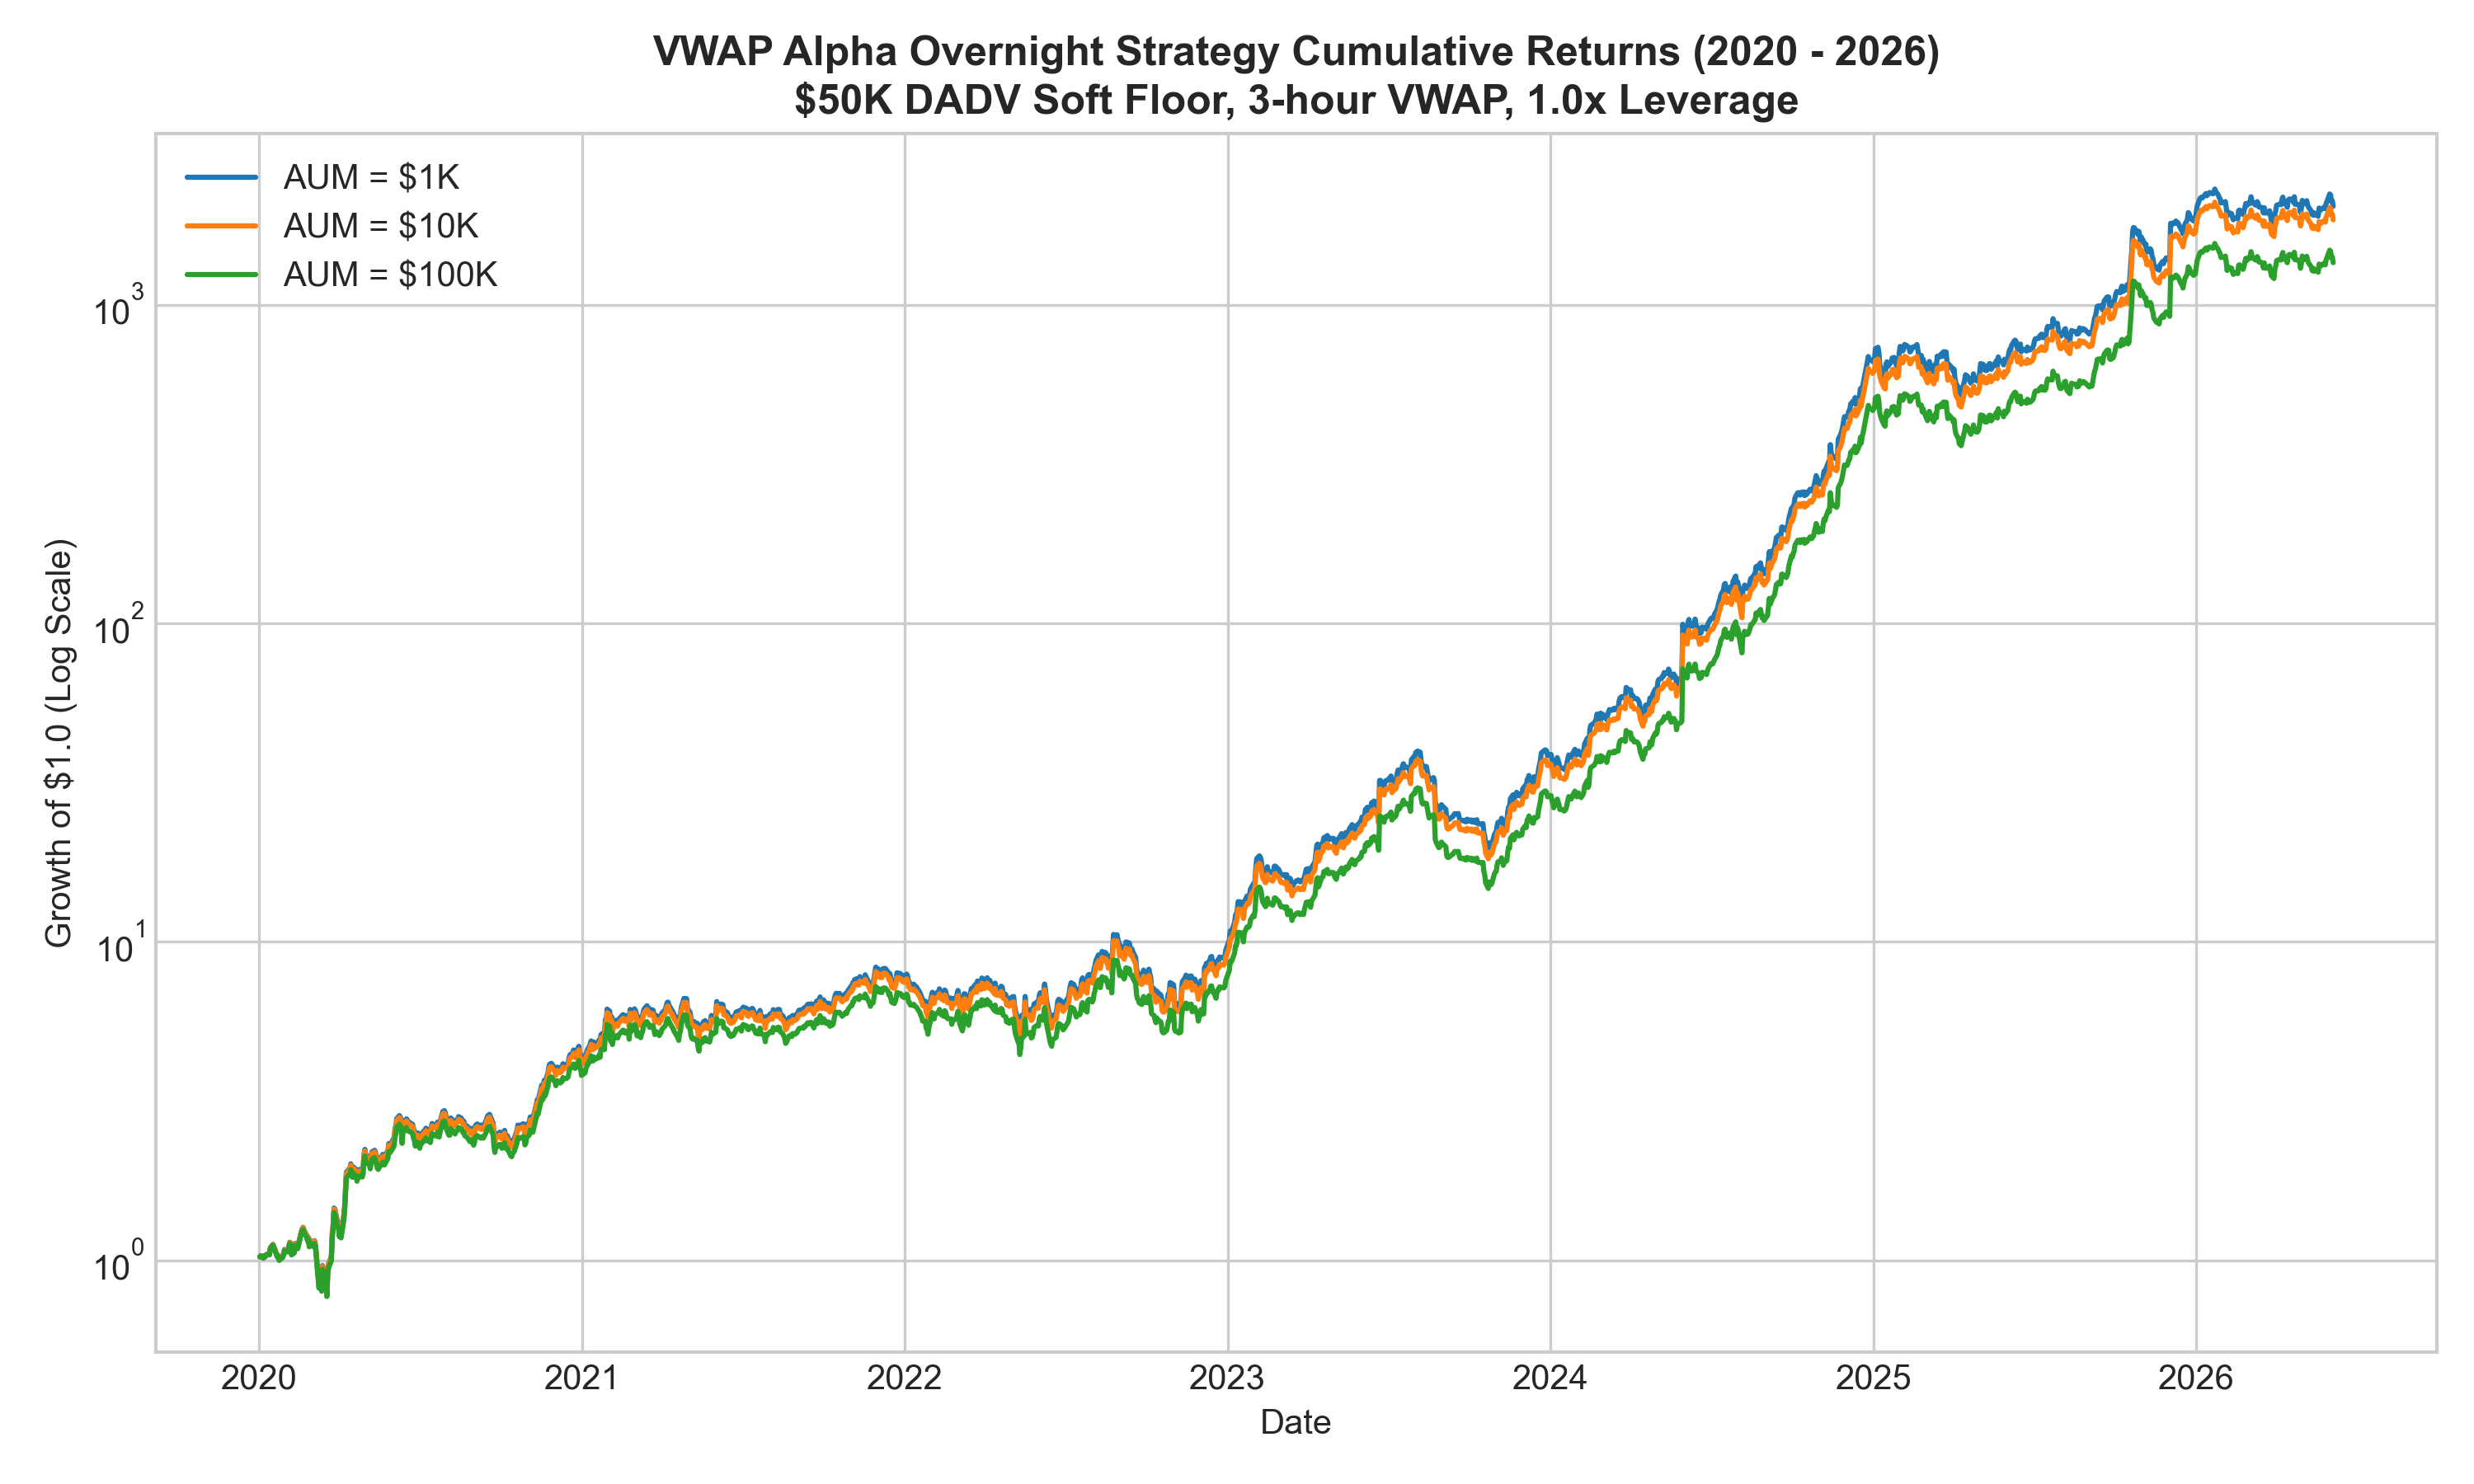
\includegraphics[width=0.85\textwidth]{pnl_chart_2020_2026.png}
\caption{Cumulative Net Returns (2020--2026)}
\label{fig:pnl_2020}
\end{figure}

\begin{figure}[htbp]
\centering
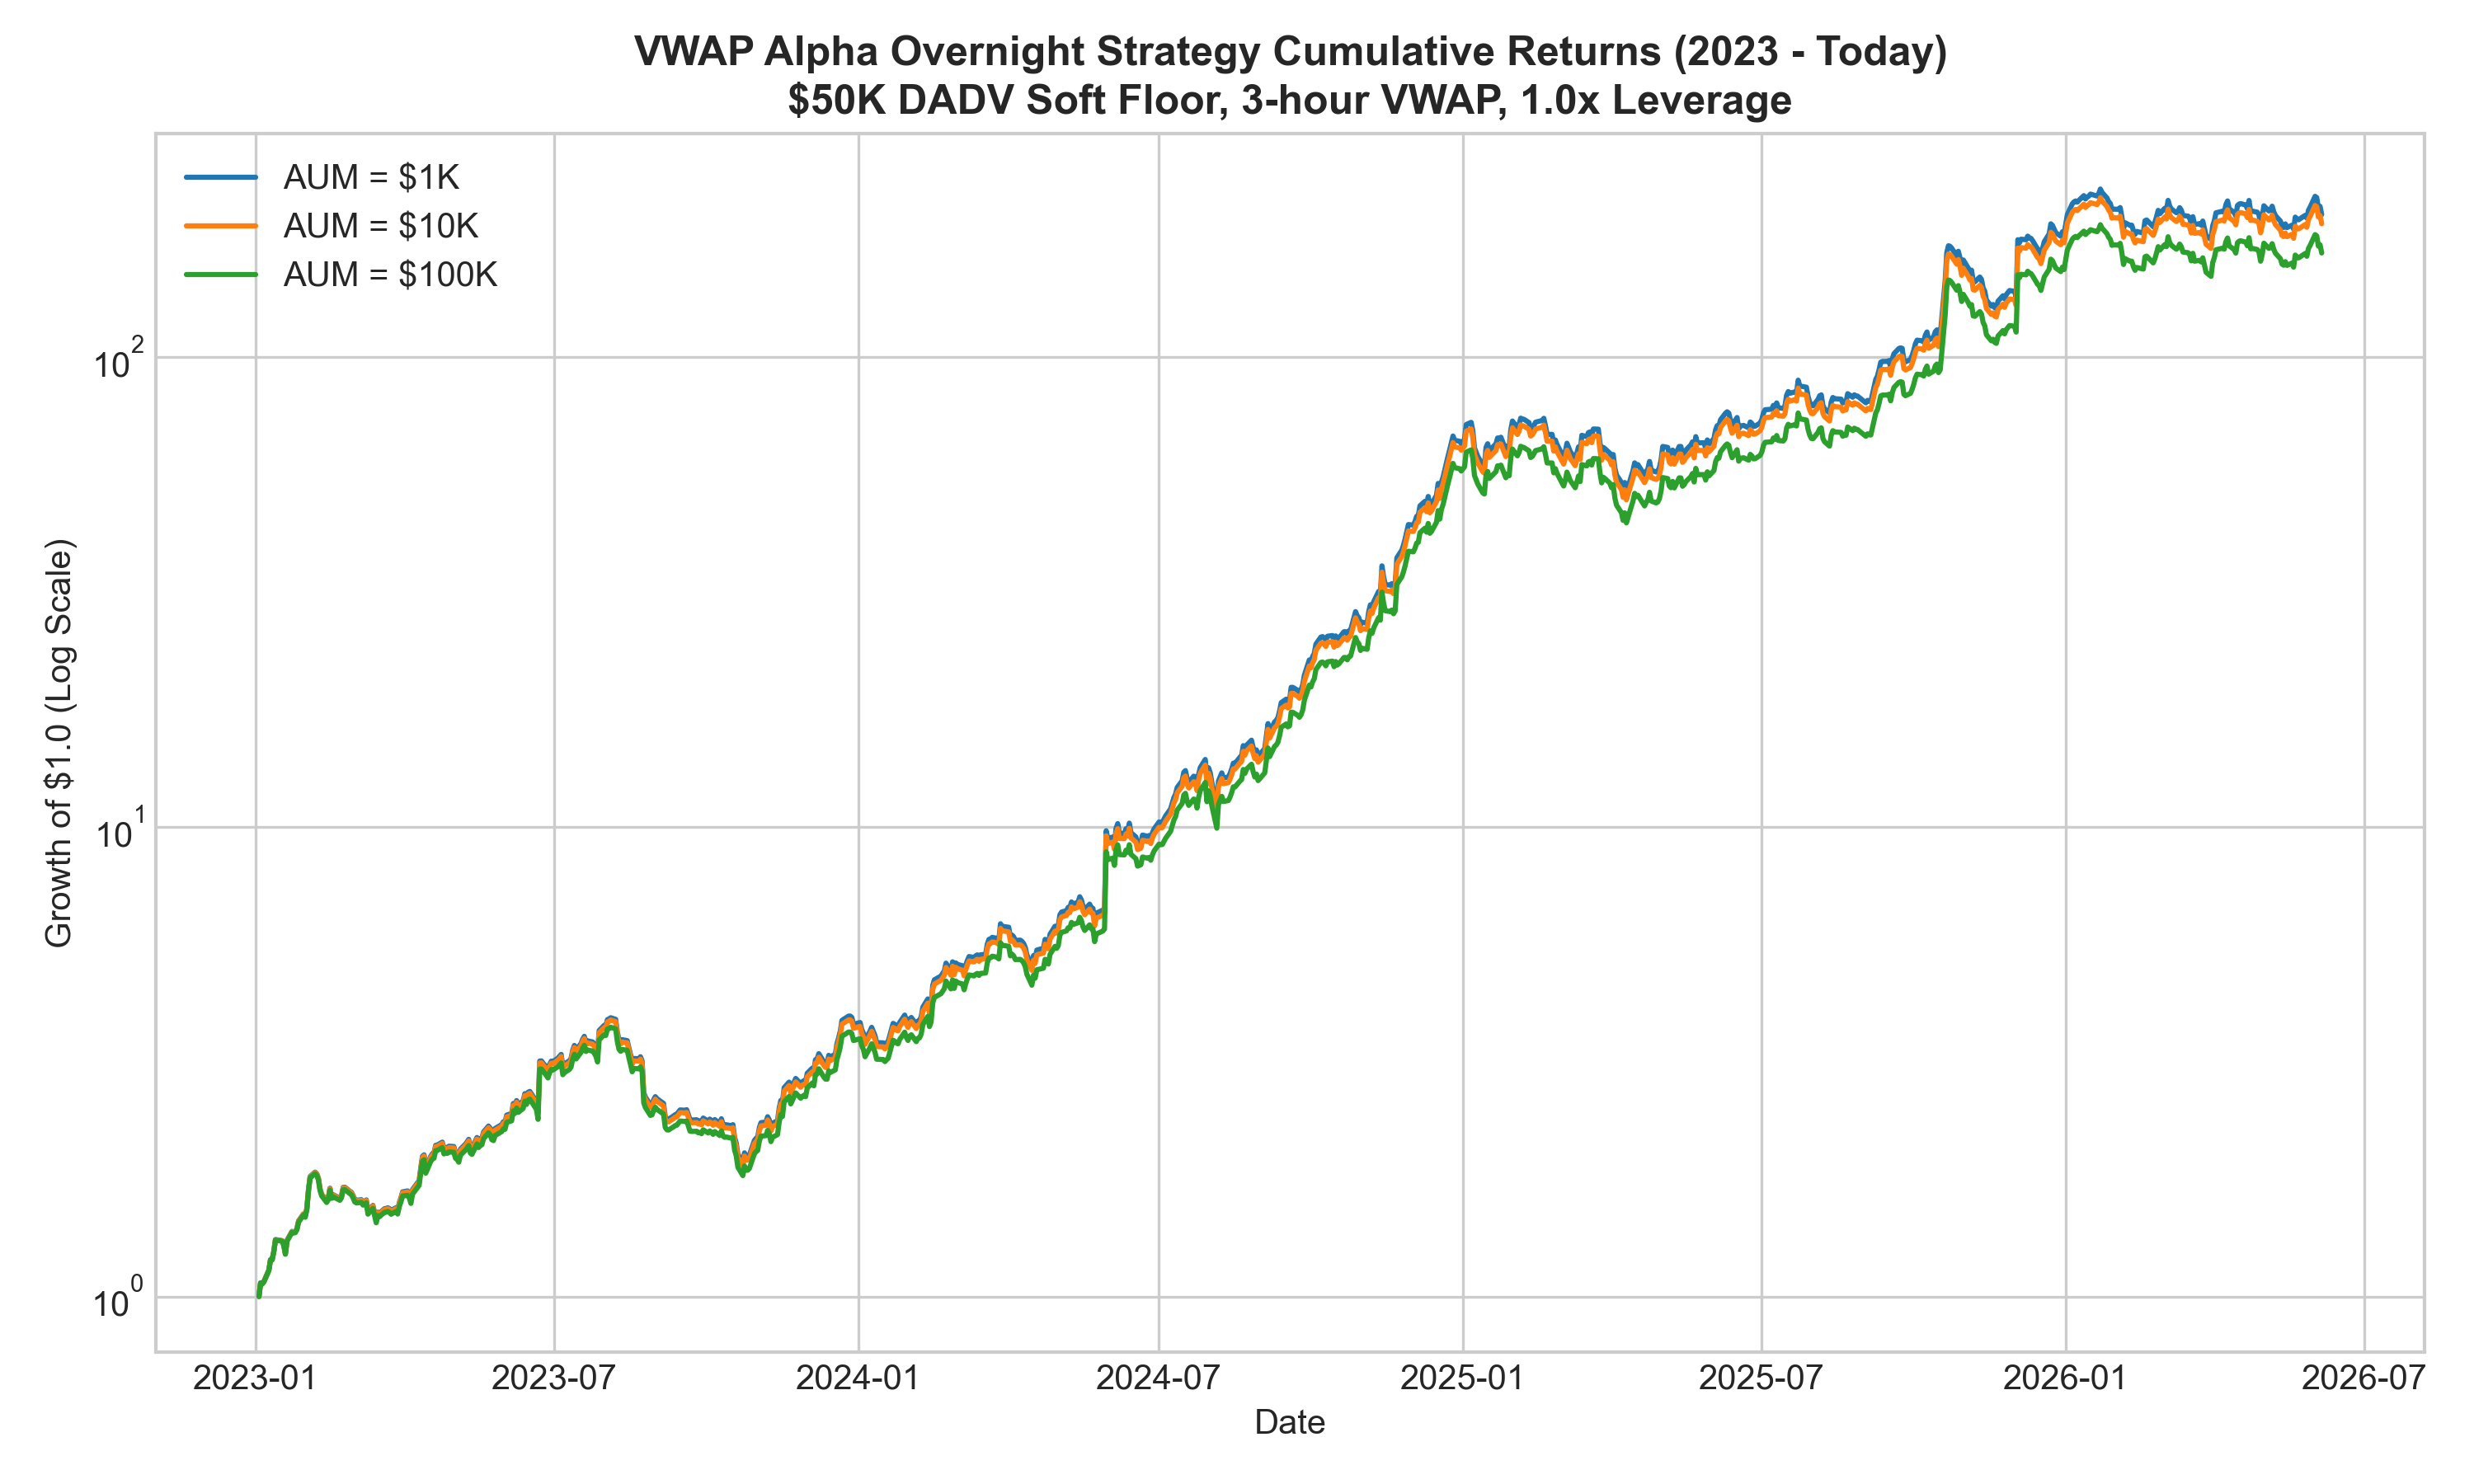
\includegraphics[width=0.85\textwidth]{pnl_chart_2023_2026.png}
\caption{Cumulative Net Returns Re-based (2023--Today)}
\label{fig:pnl_2023}
\end{figure}

\section{Robustness \& Regimes}
We evaluate the strategy's robustness across distinct sub-periods and track year-by-year performance metrics in Table \ref{tab:yearly}.

\begin{table}[htbp]
\centering
\caption{Sub-Period Sharpe Matrix (1998--2026)}
\begin{tabular}{lcccc}
\toprule
AUM Scale & Pre-Crisis (1998-2007) & Post-Crisis (2008-2019) & COVID/Modern (2020-2026) & Full Horizon \\
\midrule
\$10K & 3.348 & 2.230 & 2.355 & 2.560 \\
\$1.0M & 1.964 & 1.126 & 1.466 & 1.462 \\
\$3.0M & 1.744 & 0.903 & 1.299 & 1.260 \\
\$5.0M & 1.593 & 0.750 & 1.184 & 1.120 \\
\bottomrule
\end{tabular}
\end{table}

\begin{table}[htbp]
\centering
\caption{Year-by-Year Performance Metrics (2020--2026)}
\label{tab:yearly}
\begin{tabular}{ccccc}
\toprule
Year & Net Sharpe & Net CAGR & Max Drawdown & Trading Days \\
\midrule
2020 & 1.578 & 135.55\% & -40.36\% & 253 \\
2021 & 1.188 & 56.25\% & -23.95\% & 252 \\
2022 & 0.022 & -15.49\% & -42.21\% & 251 \\
2023 & 2.329 & 179.54\% & -52.34\% & 250 \\
2024 & 4.078 & 1325.61\% & -20.10\% & 252 \\
2025 & 1.660 & 149.87\% & -34.79\% & 250 \\
2026 & 0.672 & 22.25\% & -23.48\% & 106 \\
\bottomrule
\end{tabular}
\end{table}

\section{Conclusion}
The strategy is highly viable up to \$2.5M AUM. Operational deployment requires an initial capital of \$10K to dilute fixed ticket charges, a \$50K DADV soft floor filter, and a 3-hour VWAP execution slicing window. Monthly excess gains above \$2.5M should be swept to cash to prevent execution slippage.

\end{document}
